% C.27 ⊙O r=5, 弦 AB=8, 求 OM
\documentclass[tikz,border=4pt]{standalone}
\usepackage{ctex}
\usepackage{amsmath}
\usetikzlibrary{calc, arrows.meta}
\begin{document}
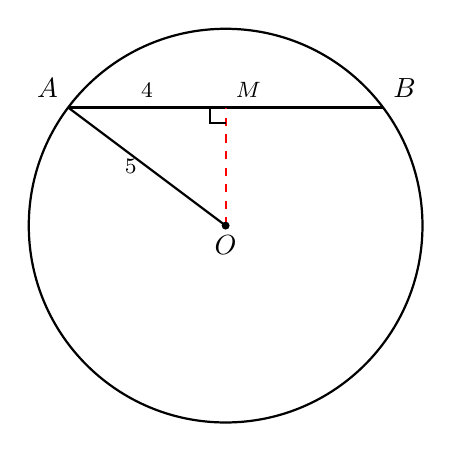
\begin{tikzpicture}[scale=0.5, thick]
  \coordinate (O) at (0,0);
  \draw (O) circle (5);
  % chord AB=8: half=4, distance OM = 3
  \coordinate (A) at (-4,3);
  \coordinate (B) at (4,3);
  \coordinate (M) at (0,3);
  \draw (A) -- (B);
  \draw[red, dashed] (O) -- (M);
  \draw (O) -- (A);
  \draw (-0.4,3) -- (-0.4,2.6) -- (0,2.6);
  \filldraw (O) circle (2pt) node[below] {$O$};
  \node[above left] at (A) {$A$};
  \node[above right] at (B) {$B$};
  \node[above right, font=\footnotesize] at (M) {$M$};
  \node[font=\footnotesize, above] at (-2,3) {$4$};
  \node[font=\footnotesize, left] at ($(O)!0.5!(A)$) {$5$};
\end{tikzpicture}
\end{document}
